


\begin{figure}[h!]%h!
    \centering
    \begin{subfigure}{.47\textwidth}
        \centering
        %\includegraphics[width=0.9\linewidth]{spec_no_shift.jpg}
        %* Figure 1
        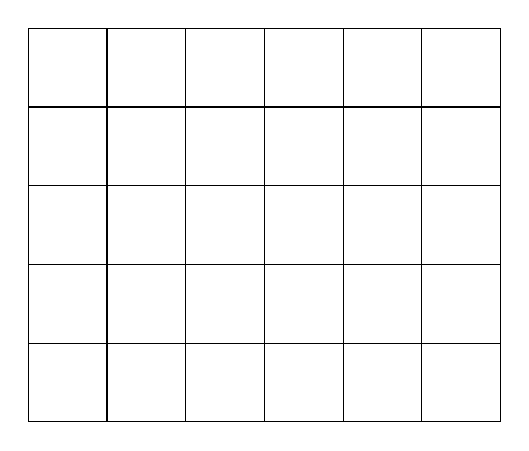
\begin{tikzpicture}[scale=1]
            % Define the tile
            \def\tile{
              % Draw the unit square
              \draw (0,0) rectangle (1,1);
            }
          
            % Draw the tiling pattern
            \foreach \x in {0,1,2,3,4,5}{
              \foreach \y in {0,1,2,3,4}{
                \pgfmathsetmacro{\shiftX}{\x} % Set horizontal shift
                \pgfmathsetmacro{\shiftY}{\y} % Set vertical shift
                \begin{scope}[shift={(\shiftX,\shiftY)}]
                  \tile % Draw the tile
                \end{scope}
              }
            }
        \end{tikzpicture}
        %* —————————————————
        \caption{Lattice tiling}
        \label{fig:tiling_one}
    \end{subfigure}\quad
    \begin{subfigure}{.47\textwidth}
        \centering
        \includegraphics[width=0.87\linewidth]{Penrose_Tiling_.png}
        \caption{P1 Penrose tiling \cite{inductiveloadP1TilingUsing}}
        \label{fig:tiling_two}
    \end{subfigure}
    \caption{Two contrasting tilings of the plane to emphasize the range of complexity. \cref{fig:tiling_one} shows a simple monohedral tiling, and \labelcref{fig:tiling_two} shows an intricate, non-periodic tiling using four different tiles. The coloring in the latter is used to distinguish the tiles more easily and highlight the three \emph{matching rules} for the pentagonal tiles, the only ones with different colors for the same shape. Matching rules are needed in order to tile aperiodically \cite{penrosePentaplexityClassNonPeriodic1979}.}
    \label{fig:tilings_one_two}
\end{figure}

% Penrose goes into the details of these in his paper 

\mycomment{  %! Block comment
The lattice tiling in \labelcref{fig:tiling_one} has fewer tiles and lacks variety compared to Penrose's original aperiodic tiling.

Two tilings of the plane to emphasize the contrast between monohedral tilings and an intricate tiling
Two tilings of the plane emphasize the contrast from monohedral tilings to more intricate tilings, such as the Penrose tiling in Fig. 

Two contrasting tilings of the plane between a monohedral tiling in \cref{fig:tiling_one} and more intricate tilings such as the Penrose tiling in \cref{fig:tiling_two} 

In contrast to the simple monohedral tiling shown in \cref{fig:tiling_one}, the Penrose tiling in \cref{fig:tiling_two} and other intricate tilings provide contrasting examples of tilings on the plane.
In contrast to the simple monohedral tiling shown in \cref{fig:tiling_one}, the Penrose tiling in \cref{fig:tiling_two} is a contrasting example of a more intricate tiling of the plane. 
In contrast to the simple monohedral tiling shown in \cref{fig:tiling_one}, the Penrose tiling in \cref{fig:tiling_two} is an example of a more intricate tiling of the plane. 

Two contrasting tilings of the plane to emphasize the stark difference between a simple monohedral tiling in \cref{fig:tiling_one} and more intricate tilings such as the Penrose tiling in \cref{fig:tiling_two}.
Two contrasting tilings of the plane to emphasize the stark difference between a simple monohedral tiling in \cref{fig:tiling_one} and a more intricate tiling in \cref{fig:tiling_two} which is non-periodic and uses four tiles. 

To emphasize the stark difference between a simple monohedral tiling in \cref{fig:tiling_one} and a more intricate tiling in \cref{fig:tiling_two} which is non-periodic and uses four tiles, we present two contrasting tilings of the plane.

Two contrasting tilings of the plane to emphasize the range of complexity. \cref{fig:tiling_one} shows a simple monohedral tiling, and \cref{fig:tiling_two} shows an intricate, non-periodic tiling using four different tiles. 
} 